\section{Model d'operacions}
\label{sec:model:sgst-operacions}

Una sèrie temporal té un atribut de temps que ha de ser tingut en
compte pels operadors que la manipulin.  Així, atenent a aquest
atribut de temps, el comportament d'una sèrie temporal pot tenir
naturaleses diferents:
\begin{itemize}
\item Conjunt, és a dir els operadors només atenen a la forma
  estructural bàsica.
\item Seqüència, en la qual els operadors la tracten com a conjunts
  amb ordre.
\item Funció temporal, en la qual els operadors treballen tenint en
  compte que una sèrie temporal és la representació d'un funció
  contínua.
\end{itemize}


En el disseny del model d'operacions següent es distingeix el
comportament per als tres casos anteriors.  Es dissenyen les
operacions bàsiques que permeten que posteriorment es combinin per
elaborar-ne de més complexes.




\subsection{Bàsiques de conjunts}

En el model estructural de SGST hem definit les sèries temporals
utilitzant conjunts. En aquest apartat definim operadors per a les
sèries temporals recollint els operadors habituals que tenen els
conjunts.

El model relacional de SGBD defineix els seus operadors bàsics a
partir de l'àlgebra de
conjunts \parencite[cap.~6]{date:introduction}. En aquest apartat
apliquem el mateix estudi per al model de SGST. Tot i així de manera
simplificada, a les definicions no es descriuen les sèries temporals
com a relacions amb capçaleres sinó que se n'escriuen només els
conjunts de valors. Seguint el model de \citeauthor{date:introduction}
es poden estendre les definicions i introduir el model complet de
relacions.


Les operacions que agrupen els elements dels conjunts habitualment se
solen representar gràficament mitjançant diagrames de Venn. A la
\autoref{fig:model:sgst:venn} es mostren els diagrames de Venn per a
cinc de les operacions dels SGSTM que descrivim a continuació:
inclusió, unió, diferència, intersecció i diferència simètrica; tant
en la seva vessant com a conjunt com en la seva vessant temporal.
\begin{figure}[tp]
  \centering
  \def\escala{0.7}

\def\nodeA{node [anchor=east] {$A$}}
\def\nodeB{node [anchor=west] {$B$}}
\def\nodeT{node [left=0.4cm] {\tiny $t_A$} node [right=0.4cm] {\tiny $t_B$}}
% Definition of circles
\def\firstcircle{(0,0) circle (1.5cm)}
\def\secondcircle{(0:2cm) circle (1.5cm)}
\def\thirdcircle{(0:1cm) circle (1.11cm)}

\colorlet{circle edge}{blue!50}
\colorlet{circle area}{blue!20}

\tikzset{
  filled/.style={fill=circle area, draw=circle edge, thick},
  outline/.style={draw=circle edge, thick},
  every node/.style={transform shape}
}

%\setlength{\parskip}{5mm}



%Set A in B
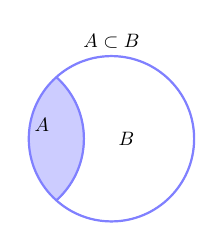
\begin{tikzpicture}[scale=\escala]
    \begin{scope}
        \clip \secondcircle;
        \draw[even odd rule,blue] \firstcircle \nodeA
                                 \secondcircle ;
                                 %\thirdcircle;
            \fill[filled] \firstcircle;
   \end{scope}
      \draw[outline] \secondcircle \nodeB;

   \node[anchor=south] at (current bounding box.north) {$A \subset B$};
   \node[anchor=west] at (current bounding box.west) {$A$};
\end{tikzpicture}
%Set temporal A in B
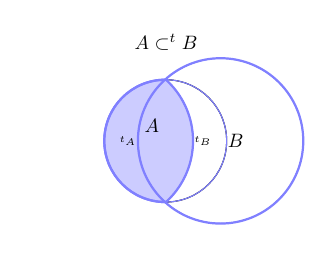
\begin{tikzpicture}[scale=\escala]
    \begin{scope}
        \clip \firstcircle;
        \fill[filled] \thirdcircle;
      \draw[outline] \thirdcircle \nodeT;
    \end{scope}
    \begin{scope}
        \clip \secondcircle;
        \draw \thirdcircle \nodeT;
    \end{scope}
      \draw[circle edge] \thirdcircle;
    \begin{scope}
        \clip \secondcircle;
        \draw[even odd rule,blue] \firstcircle \nodeA
                                 \secondcircle ;
                                 %\thirdcircle;
            \draw[outline] \firstcircle;
   \end{scope}
      \draw[outline] \secondcircle \nodeB;

   \node[anchor=south] at (current bounding box.north) {$A \subset^t B$};
   \node[anchor=east] at (current bounding box.center) {$A$};
\end{tikzpicture}







%Set A or B
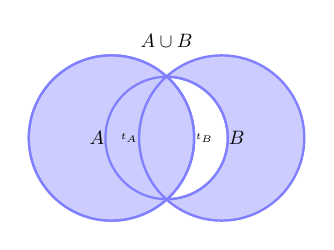
\begin{tikzpicture}[scale=\escala]
  \draw[filled] \firstcircle \nodeA;
    \begin{scope}
        \clip \secondcircle;
        \draw[filled, even odd rule] \firstcircle \nodeA
                                 \secondcircle 
                                 \thirdcircle;
   \end{scope}
    \draw[outline] \firstcircle
                   \secondcircle \nodeB
                   \thirdcircle \nodeT;

   \node[anchor=south] at (current bounding box.north) {$A \cup B$};
\end{tikzpicture}
%Set temporal A or B
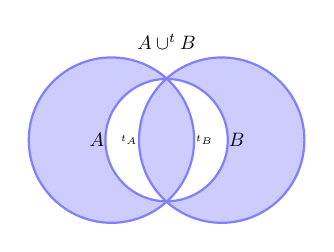
\begin{tikzpicture}[scale=\escala]
    \draw[filled, even odd rule] \firstcircle \nodeA
                                 \secondcircle \nodeB
                                 \thirdcircle \nodeT;
    \node[anchor=south] at (current bounding box.north) {$A \cup^t B$};
\end{tikzpicture}




% Set A but not B
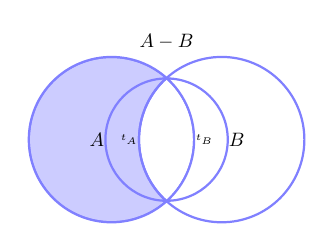
\begin{tikzpicture}[scale=\escala]
    \begin{scope}
        \clip \firstcircle;
        \draw[filled, even odd rule] \firstcircle \nodeA
                                     \secondcircle;

    \end{scope}
    \draw[outline] \firstcircle
                   \secondcircle \nodeB
                   \thirdcircle \nodeT;
    \node[anchor=south] at (current bounding box.north) {$A - B$};
\end{tikzpicture}
% Set temporal A but not B
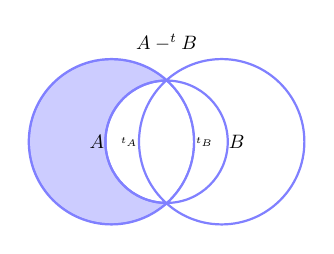
\begin{tikzpicture}[scale=\escala]
    \begin{scope}
        \clip \firstcircle;
        \draw[filled, even odd rule] \firstcircle \nodeA
                                     \thirdcircle;

    \end{scope}
    \draw[outline] \firstcircle
                   \secondcircle \nodeB
                   \thirdcircle \nodeT;
    \node[anchor=south] at (current bounding box.north) {$A -^t B$};
\end{tikzpicture}





% % Set A and B
% \begin{tikzpicture}
%     \begin{scope}
%         \clip \firstcircle;
%         \fill[filled] \secondcircle;
%     \end{scope}
%     \draw[outline] \firstcircle \nodeA;
%     \draw[outline] \secondcircle \nodeB;
%     \draw[outline] \thirdcircle \nodeT;
%     \node[anchor=south] at (current bounding box.north) {$A \cap B$};
% \end{tikzpicture}
% % Set temporal A and B
% \begin{tikzpicture}
%     \begin{scope}
%         \clip \firstcircle;
%         \fill[filled] \thirdcircle;
%     \end{scope}
%     \draw[outline] \firstcircle \nodeA;
%     \draw[outline] \secondcircle \nodeB;
%     \draw[outline] \thirdcircle \nodeT;
%     \node[anchor=south] at (current bounding box.north) {$A \cap^t B$};
% \end{tikzpicture}



% %Set A or B but not (A and B) also known a A xor B
% \begin{tikzpicture}
%     \begin{scope}
%         \clip \firstcircle;
%         \draw[filled, even odd rule] \firstcircle
%                                      \secondcircle;
%     \end{scope}
%     \begin{scope}
%         \clip \secondcircle;
%         \draw[filled, even odd rule] \secondcircle 
%                                      \thirdcircle;

%     \end{scope}
%     \draw[outline] \firstcircle \nodeA;
%     \draw[outline] \secondcircle \nodeB;
%     \draw[outline] \thirdcircle \nodeT;
%     \node[anchor=south] at (current bounding box.north) {$A \ominus B$};
% \end{tikzpicture}
% %Set temporal A or B but not (A and B) also known a A xor B
% \begin{tikzpicture}
%     \begin{scope}
%         \clip \firstcircle;
%         \draw[filled, even odd rule] \firstcircle
%                                      \thirdcircle;
%     \end{scope}
%     \begin{scope}
%         \clip \secondcircle;
%         \draw[filled, even odd rule] \secondcircle 
%                                      \thirdcircle;

%     \end{scope}
%     \draw[outline] \firstcircle \nodeA;
%     \draw[outline] \secondcircle \nodeB;
%     \draw[outline] \thirdcircle \nodeT;
%     \node[anchor=south] at (current bounding box.north) {$A \ominus^t B$};
% \end{tikzpicture}
  \caption{Diagrames de Venn per a les operacions dels SGSTM. Els
    subconjunts $t_a$ i $t_b$ indiquen les mesures que comparteixen el
    mateix temps amb una altra mesura de l'altre conjunt però no el
    mateix valor.}
  \label{fig:model:sgst:venn}
\end{figure}


\subsubsection{Pertinença i inclusió}

La pertinença determina si un element pertany a un conjunt.  Sigui
$S=\{m_0,\ldots,m_k\}$ una sèrie temporal i $m$ una mesura, es
defineix de la mateixa manera que en els conjunts la pertinença de la
mesura a la sèrie temporal $m \in S$. Atenent a l'atribut de temps, es
defineix la pertinença temporal d'una mesura a una sèrie temporal.
\begin{definition}[Pertinença temporal]
  Sigui $S=\{m_0,\ldots,m_k\}$ una sèrie temporal i $m=(t,v)$ una
  mesura.  Direm que la mesura pertany temporalment a la sèrie
  temporal $m \inst S$ si i només si $\exists m_a \in S : T(m) =
  T(m_a)$.
\end{definition}


La inclusió determina si tots els elements d'un conjunt pertanyen a un
altre conjunt. Siguin $S_1=\{m_0^1,\ldots,m_k^1\}$ i
$S_2=\{m_0^2,\ldots,m_l^2\}$ dues sèries temporals, la primera sèrie
temporal està inclosa en la segona $S_1 \subseteq S_2$ si $\forall m
\in S_1: m \in S_2$. Aleshores, $S_1$ és una subsèrie temporal de
$S_2$. Aquesta definició d'inclusió determina un ordre parcial entre
les sèries temporals.



\subsubsection{Màxim i suprem}

La relació definida a~\ref{def:model:mesura-relacio-ordre} indueix
sobre una sèrie temporal una relació d'ordre total. Com que la sèrie
temporal s'ha considerat finita i sense elements repetits, quan la
sèrie temporal no és buida això comporta l'existència d'un màxim i
d'un mínim.  Si $S$ és una sèrie temporal, $\max(S)$ i $\min(S)$ són
respectivament la mesura màxima i mínima d'$S$.

\begin{definition}[Màxim i mínim]
  Sigui $S=\{m_0,\ldots,m_k\}$ una sèrie temporal i $n\in S$ una
  mesura.  Direm que $n=\max(S)$ és el màxim de la sèrie temporal si i
  només si $\forall m \in S: n \geq m $.  Direm que $n=\min(S)$ és el
  mínim de la sèrie temporal si i només si $\forall m \in S: n \leq
  m$.
\end{definition}

El $\max(S)$ i el $\min(S)$ no estan definits quan la sèrie temporal
és buida: $S= \emptyset$. En
canvi, el suprem i l'ínfim estan definits per qualsevol
sèrie temporal tal com passa amb el conjunt estès de nombres reals,
\cite{cantrell:extendedreal}.  

\begin{definition}[Suprem i ínfim]\label{def:sgst:sup}\label{def:sgst:inf}
  Sigui $S=\{m_0,\ldots,m_k\}$ una sèrie temporal i $n\in S$ una
  mesura.  Direm que $n=\sup(S)$ és el suprem de la sèrie temporal si
  $n=\max(S)$ en cas que el màxim estigui definit o
  $n=(-\infty,\infty)$ en cas contrari.  Direm que $n=\inf(S)$ és
  l'ínfim de la sèrie temporal si $n=\min(S)$ en cas que el mínim
  estigui definit o $n=(+\infty,\infty)$ en cas contrari.
\end{definition}

Quan la sèrie temporal no és buida, per
ser un conjunt finit i d'ordre total, sempre hi ha un i només un màxim
i un mínim i per tant es corresponen amb el suprem i l'ínfim
respectivament.




\subsubsection{Unió}

La unió de dos conjunts és un conjunt que conté tots els elements
d'ambdós conjunts.  Per a poder unir dos conjunts amb estructura de
relació, $A \cup B$, cal que tots dos tinguin la mateixa estructura;
és a dir, en termes de SGBDR cal que $A$ i $B$ tinguin la mateixa
capçalera.

Per tal que l'operació d'unió de conjunts sigui vàlida per a les
sèries temporals cal, a més, tenir en compte quan dues sèries
temporals tenen mesures en el mateix instant de temps. En cas
d'utilitzar l'operació d'unió de conjunts la sèrie temporal resultant
no compliria amb la definició \ref{def:serie_temporal} ja que
contindria mesures amb temps repetits. Com a conseqüència, es
defineixen dues operacions d'unió per a les sèries temporals que
resolen la restricció del temps de forma diferent.

En primer lloc, es defineix la unió de dues sèries temporals que
escull les mesures del primer operand en cas de mesures repetides.
\begin{definition}[unió]
  Sigui $S_1=\{m_0^1, \dotsc, m_{k_1}^1\}$ i $S_2=\{m_0^2, \dotsc,
  m_{k_2}^2\}$ dues sèries temporals, la unió de les dues
  sèries temporals $S_1 \cup S_2$ és una sèrie temporal $S=\{m_0,
  \dotsc, m_k\}$ que conté totes les mesures de $S_1$ i les mesures de
  $S_2$ no repetides: $S_1 \cup S_2 = \{m^1 \in S_1 \vee m^2 \in S_2
  | m^2 \notinst S_1 \}$.
\end{definition}

Propietats de la unió de sèries temporals:
\begin{itemize}
\item La dimensió $k$ de la sèrie temporal resultant està fitada a
  $k_1 \leq k \leq k_1 + k_2$. 
\item No commutativa. En general
  $S_1\cup S_2 \neq S_2\cup S_1$ tot i que sí que es compleix
  l'equivalència respecte al cardinal $|S_1 \cup S_2| = |S_2\cup S_1|$.
\end{itemize}

En segon lloc, es defineix la unió temporal de dues sèries temporals
que és la unió sense tenir en compte les mesures que tenen el mateix
instant de temps i diferent valor.
\begin{definition}[unió temporal]
  Sigui $S_1=\{m_0^1, \dotsc, m_{k_1}^1\}$ i $S_2=\{m_0^2, \dotsc,
  m_{k_2}^2\}$ dues sèries temporals, la unió temporal de les dues
  sèries temporals $S_1 \cupt S_2$ és una sèrie temporal $S=\{m_0,
  \dotsc, m_k\}$ que conté les mesures de $S_1$ i de $S_2$ excloent
  les que només comparteixen el temps: $S_1 \cupt S_2 = \{ m^1 \in S_1
  \vee m^2 \in S_2 | m^1 \notinst S_2 \vee m^1 \in S_2, m^2 \notinst
  S_1 \}$.
\end{definition}


Propietats de la unió temporal:
\begin{itemize}
\item Commutativa
\end{itemize}



\subsubsection{Diferència}

La diferència de dos conjunts és un conjunt que conté tots els
elements del primer conjunt que no pertanyen al segon.  Per a poder
restar dos conjunts amb estructura de relació, $A - B$, cal que
tots dos tinguin la mateixa estructura; és a dir, en termes de SGBDR
cal que $A$ i $B$ tinguin la mateixa capçalera.

En la definició de l'operació de diferència cal tenir en compte les
dues pertinences possibles.

En primer lloc, es defineix la diferència atenent a la pertinença
estricta de conjunts. És a dir s'aplica la diferència de
conjunts a les sèries temporals.
\begin{definition}[diferència]
  Sigui $S_1=\{m_0^1, \dotsc, m_{k_1}^1\}$ i $S_2=\{m_0^2, \dotsc,
  m_{k_2}^2\}$ dues sèries temporals, la diferència de les dues
  sèries temporals $S_1 - S_2$ és una sèrie temporal $S=\{m_0,
  \dotsc, m_k\}$ que conté totes les mesures de $S_1$ que no pertanyen a
  $S_2$: $S_1 - S_2 = \{ m \in S_1 | m \notin S_2  \}$.
\end{definition}

En segon lloc, es defineix la diferència atenent a la pertinença
temporal.
\begin{definition}[diferència temporal]
  Sigui $S_1=\{m_0^1, \dotsc, m_{k_1}^1\}$ i $S_2=\{m_0^2, \dotsc,
  m_{k_2}^2\}$ dues sèries temporals, la diferència temporal de les
  dues sèries temporals $S_1 -^t S_2$ és una sèrie temporal
  $S=\{m_0, \dotsc, m_k\}$ que conté totes les mesures de $S_1$ que no
  pertanyen temporalment a $S_2$: $S_1 -^t S_2 = \{ m \in S_1 | m
  \notinst S_2 \}$.
\end{definition}




\subsubsection{Intersecció}

La intersecció de dos conjunts és un conjunt que conté els elements
comuns als dos conjunts.  Per a poder intersecar dos conjunts amb estructura
de relació, $A \cap B$, cal que tots dos tinguin la mateixa
estructura; és a dir, en termes de SGBDR cal que $A$ i $B$ tinguin la
mateixa capçalera.

En la definició de l'operació d'intersecció cal tenir en compte les
dues pertinences possibles.

En primer lloc, es defineix la diferència atenent a la pertinença
estricta de conjunts. És a dir s'aplica l'operació d'intersecció de
conjunts.
\begin{definition}[intersecció]
  Sigui $S_1=\{m_0^1, \dotsc, m_{k_1}^1\}$ i $S_2=\{m_0^2, \dotsc,
  m_{k_2}^2\}$ dues sèries temporals, la intersecció de les dues
  sèries temporals $S_1 \cap S_2$ és una sèrie temporal $S=\{m_0,
  \dotsc, m_k\}$ que conté les mesures de $S_1$ repetides a $S_2$:
  $S_1 \cap S_2 = \{ m \in S_1 | m \in S_2 \}$.
\end{definition}

En segon lloc, es defineix la intersecció atenent a la pertinença
temporal tenint en compte quan dues sèries temporals tenen mesures en
el mateix instant de temps però de valor diferent.
\begin{definition}[intersecció temporal]
  Sigui $S_1=\{m_0^1, \dotsc, m_{k_1}^1\}$ i $S_2=\{m_0^2, \dotsc,
  m_{k_2}^2\}$ dues sèries temporals, la intersecció temporal de les
  dues sèries temporals $S_1 \capt S_2$ és una sèrie temporal
  $S=\{m_0, \dotsc, m_k\}$ que conté les mesures de $S_1$ repetides
  temporalment a $S_2$: $S_1 \capt S_2 = \{ m \in S_1 | m \inst S_2
  \}$.
\end{definition}

Propietats de la intersecció:
\begin{itemize}
\item La intersecció és commutativa però la intersecció temporal no és
  commutativa.
\item A partir de la diferència es pot definir la intersecció: $S_1
  \cap S_2 \equiv S_1 - (S_1 - S_2)$.
\end{itemize}


\subsubsection{Diferència simètrica}

La diferència simètrica de dos conjunts és un conjunt que conté els
elements no comuns dels dos conjunts. La diferència simètrica de dos
conjunts $A \ominus B$ es defineix a partir de la diferència i la
unió:
\begin{align*}
A \ominus B  & \equiv (A-B)\cup(B-A)\\
             & \equiv (A\cup B)-(A\cap B)  \\
A \ominus B  & \subseteq A\cup B
\end{align*}

Seguint aquestes propietats es defineixen dues diferències
simètriques: una a partir de la diferència i la unió de sèries
temporals i una altra a partir de la diferència temporal i la unió
temporal.  Per tal que l'operació de diferència simètrica sigui vàlida
per a les sèries temporals cal tenir en compte quan dues sèries
temporals tenen mesures en el mateix instant de temps.

En primer lloc, es defineix la diferència simètrica excloent les
mesures amb el mateix temps però de valor diferent.
\begin{definition}[diferència simètrica]
  Sigui $S_1=\{m_0^1, \dotsc, m_{k_1}^1\}$ i $S_2=\{m_0^2, \dotsc,
  m_{k_2}^2\}$ dues sèries temporals, la diferència simètrica de les
  dues sèries temporals $S_1 \ominus S_2$ és una sèrie temporal
  $S=\{m_0, \dotsc, m_k\}$ que conté les mesures de $S_1$ o
  exclusivament les de $S_2$: $S_1 \ominus S_2 = \{ m^1 \in S_1 \vee
  m^2 \in S_2 | m^1 \notinst S_2, m^2 \notin S_1 \}$.
\end{definition}

En segon lloc, es defineix la diferència simètrica temporal excloent les
mesures amb el mateix temps.
\begin{definition}[diferència simètrica temporal]
  Sigui $S_1=\{m_0^1, \dotsc, m_{k_1}^1\}$ i $S_2=\{m_0^2, \dotsc,
  m_{k_2}^2\}$ dues sèries temporals, la diferència simètrica de les
  dues sèries temporals $S_1 \ominus S_2$ és una sèrie temporal
  $S=\{m_0, \dotsc, m_k\}$ que conté les mesures de $S_1$ o
  exclusivament les de $S_2$: $S_1 \ominus S_2 = \{ m^1 \in S_1 \vee
  m^2 \in S_2 | m^1 \notinst S_2, m^2 \notinst S_1 \}$.
\end{definition}



\subsubsection{Projecció}

La projecció és una operació dels SGBDR que selecciona uns atributs
determinats d'un conjunt. Es pot aplicar la projecció a les sèries
temporals de la mateixa manera que als
SGBDR \parencite{date:introduction}. 

Sigui $S =\{m_0, \dotsc, m_k\}$ una sèrie temporal i $A=\{a_0, \dotsc,
a_n\}$ un conjunt de noms d'atributs, la projecció de $S$ en $A$
s'escriu com $S\{a_0, \dotsc, a_n\}$.




\subsubsection{Selecció}

La selecció és una operació dels SGBDR que selecciona uns tuples
determinats d'un conjunt. Es pot aplicar la selecció a les sèries
temporals de la mateixa manera que als
SGBDR \parencite{date:introduction}. 

Sigui $S =\{m_0, \dotsc, m_k\}$ una sèrie temporal, $a_1$ i $a_2$ dos
noms d'atributs que pertanyen a $S$, i $a_1 \Theta a_2$ una expressió
booleana sobre $a_1$ i $a_2$, la selecció de $S$ per l'expressió
booleana s'escriu com $S \where a_1 \Theta a_2$.


\subsubsection{Reanomena}

El reanomena és una operació dels SGBDR que canvia el nom dels
atributs. Es pot aplicar el reanomena les sèries temporals de la
mateixa manera que als SGBDR \parencite{date:introduction}.

Sigui $S =\{m_0, \dotsc, m_k\}$ una sèrie temporal, $a$ un nom
d'atribut que pertany a $S$ i $b$ un que no hi pertany, el reanomenat
de $a$ per $b$ s'escriu com $S \rename a \as b$.





\subsubsection{Producte i junció}

El producte cartesià de dos conjunts és un conjunt que conté totes les
parelles possibles d'elements d'ambdós conjunts.  Per a poder
multiplicar dos conjunts amb estructura de relació, $A \times B$, en
termes de SGBDR cal que $A$ i $B$ no tinguin en comú noms d'atributs.
En els SGBDR, a diferència del producte de conjunts, el conjunt
resultant no és un conjunt de parells de tuples sinó un conjunt de
tuples.

\todo{} Definim el producte de dues sèries temporals, les qual en
forma canònica tinguin els atributs $t$ i $v$, com una sèrie temporal
amb atributs $t_1$, $v_1$, $t_2$ i $v_2$. Així doncs, per a sèries
temporals el producte resulta en una sèrie temporals amb dos atributs
de temps. Per aquest fet l'anomenem sèrie temporal doble
(v.\ \autoref{def:sgst:st-doble}).
\begin{definition}[producte]
  Sigui $S_1=\{m_0^1, \dotsc, m_{k_1}^1\}$ i $S_2=\{m_0^2, \dotsc,
  m_{k_2}^2\}$ dues sèries temporals en forma canònica, el producte de
  les dues sèries temporals $S_1 \times S_2$ és una sèrie temporal
  doble $S=\{m_0, \dotsc, m_k\}$ que conté la unió de totes les
  parelles de mesures de $S_1$ i $S_2$: $S_1 \times S_2 = \{
  (t_1,v_1,t_2,v_2) | (t_1,v_1) \in S_1 \wedge (t_2,v_2) \in S_2 \}$
\end{definition}

Propietats del producte:
\begin{itemize}
\item El cardinal resultant és $|S|=k_1k_2$
\item El grau resultant és $4$
\end{itemize}



La junció (\emph{join}) de dos conjunts és un conjunt que conté les
parelles d'elements d'ambdós conjunts que tenen el mateix valor per
als atributs comuns.  La junció de dos conjunts amb estructura de
relació, $A \join B$, es defineix com una selecció sobre el
producte \parencite{date:introduction}.


Per a les sèries temporals, definim la junció com l'ajuntament de les
parelles que tenen el mateix atribut de temps en ambdues sèries
temporals . El resultat de la junció és una sèrie temporal
multivaluada.
\begin{definition}[junció]\label{def:sgst:join}
  Sigui $S_1=\{m_0^1, \dotsc, m_{k_1}^1\}$ i $S_2=\{m_0^2, \dotsc,
  m_{k_2}^2\}$ dues sèries temporals en forma canònica, la junció de
  les dues sèries temporals $S_1 \join S_2$ és una sèrie temporal
  multivaluada $S=\{m_0, \dotsc, m_k\}$ que selecciona del producte de
  $S_1$ amb $S_2$ les mesures dobles amb temps iguals: $S_1 \join S_2
  = \{ (t,v_1,v_2) | (t_1,v_1,t_2,v_2) \in S_1\times S_2 \wedge
  t=t_1=t_2 \}$.
\end{definition}


Propietats de la junció:
\begin{itemize}
\item El cardinal resultant és $|S|\leq\min(k_1,k_2)$
\item És commutativa; tenint en compte que els atributs tenen nom i
  per tant l'ordre no importa.
\end{itemize}







\subsubsection{Computacionals: mapa, agregat i plec}

Per a poder operar amb els conjunts, a més de l'àlgebra definida fins
ara, es necessiten operadors amb funcionalitats computacionals; és a
dir, operadors que calculin amb els valors continguts en els conjunts. 

En els SGBDR els operadors computacionals bàsics són \emph{extend},
\emph{aggregate} i \emph{summarize} \parencite{date:introduction}.
Per a les sèries temporals definim operacions equivalents a les dues
primeres de la manera amb que habitualment s'utilitzen per als
conjunts. La tercera, el \emph{summarize}, és una operació creada a
partir de les altres dues que s'utilitza per a sintetitzar per grups i
per tant en les sèries temporals no té sentit perquè l'atribut temps
d'una sèrie temporal no pot tenir instants repetits i per tant no se'n
poden fer grups d'instants compartits.
% No obstant, es pot aplicar el \emph{summarize} per a l'atribut de
% valors: summarize S per S {v} add ...  però això ja no mapa a una
% sèrie temporal.

% De l'operador \emph{aggregate} dels SGBDR definit per
% \textcite{date:introduction} cal tenir en compte que en defineix
% dues vessants. Per una banda, defineix els \emph{aggregate operator
% invocation} que retornen valors escalars. Per altra banda, defineix
% els \emph{aggregate operator invocation} que serveixen per a
% treballar amb el \emph{summarize}.

Així doncs, a continuació es defineix l'operador mapa (\emph{map}) com
a equivalent a l'\emph{extend}, l'operador agregat (\emph{aggregate})
com a equivalent a l'\emph{aggregate} i l'operador plec (\emph{fold})
com una forma més general de calcular recursivament amb les mesures
que l'\emph{aggregate}.




L'operació de mapatge aplica una funció a cada element del conjunt.
\begin{definition}[mapa]
  Sigui $S=\{m_0, \dotsc, m_k\}$ una sèrie temporal i $f$ una funció
  sobre una mesura a on $f:m\mapsto m'$, el mapa de $f$ a $S$ és una
  sèrie temporal $S'=\{m_0', \dotsc, m_k'\}$ amb la funció aplicada a
  cada mesura: $\map(S,f) = \{\forall m\in S : f(m) \}$.
\end{definition}


L'operació d'agregació agrupa en una mesura els elements del conjunt
segons un criteri, per exemple estadístics.
\begin{definition}[agregat]
  Sigui $S=\{m_0, \dotsc, m_k\}$ una sèrie temporal, $m_i$ una mesura
  i $f$ una funció de dues mesures a on $f: m_a \times m_b \mapsto
  m_r$, l'agregat de $S$ segons $f$ amb valor inicial $m_i$ és una
  mesura $m' = (t',v')$ amb l'agrupament de les mesures seguint el
  criteri de la funció: $\agg(S,m_i,f) = f(\dots(
  f(f(f(m_i,m_0),m_1),\allowbreak m_2 )\dots),\allowbreak m_k)$.
\end{definition}

% Més compactament descrit amb
% \begin{align*}
%   \text{fold}: & S=\{m_0,\dotsc,m_k\} \times m_i \times f \longrightarrow m'= \\
%   & \begin{cases}
%     m_i & \text{si} |S|=0, \\
%     \text{fold}(S_1,f(m_i,m_1),f) & \text{altrament}
%   \end{cases}\\
%   \text{ a on } & m_1 \in S, S_1 = S - \{m_1\}
% \end{align*}


L'operació de plegament combina recursivament els elements del conjunt
segons un criteri.
\begin{definition}[plec]
  Sigui $S=\{m_0, \dotsc, m_k\}$ i $S_i=\{m_{i0}, \dotsc, m_{ik}\}$
  dues sèries temporals i $f$ una funció d'una mesura amb una sèrie
  temporal a on $f: S_a \times m_b \mapsto S_r$, el plec de $S$ segons
  $f$ amb valor inicial $S_i$ és una sèrie temporal $S'= \{m_0',
  \dotsc, m_k'\}$ amb l'agrupament de les mesures seguint el criteri
  de la funció: $\fold(S,S_i,f) = f(\dots(
  f(f(f(S_i,m_0),m_1),\allowbreak m_2 )\dots),\allowbreak m_k)$.
\end{definition}


Les operacions d'agregació i plegament tal com s'han definit es
realitzen en ordre aleatori de mesures. Segons el criteri que
s'utilitzi, l'ordre és important i per tant cal una operació que
computi tenint-lo en compte. A tal efecte, a continuació s'amplia la
funció de plegament. Per a la funció d'agregació es pot aplicar el
mateix concepte d'ordre.
\begin{definition}[plec amb ordre]
  Sigui $S=\{m_0, \dotsc, m_k\}$ i $S_i=\{m_{i0}, \dotsc, m_{ik}\}$
  dues sèries temporals, $f$ una funció d'una mesura amb una sèrie
  temporal a on $f: S_a \times m_b \mapsto S_r$ i $o$ una funció que
  treu una mesura d'una sèrie temporal a on $o: S_c \mapsto m_c$, el
  plec de $S$ segons $f$ amb valor inicial $S_i$ i ordre $o$ és una
  sèrie temporal $S'= \{m_0', \dotsc, m_k'\}$ amb l'agrupament de les
  mesures seguint el criteri i l'ordre de les funcions:
  $\fold(S,S_i,f,o) =
  \begin{cases}
    S_i & \text{si } |S|=0, \\
    \fold(S_o,f(S_i,m_o),f,o) & \text{altrament}
  \end{cases}$ a on $m_o = o(S)$ i $S_o = S - \{m_o\}$.
\end{definition}

El plec amb ordre és necessari quan la funció $f$ no és associativa ni
commutativa perquè llavors l'ordre dels càlculs importa. Es pot
observar que el plec sense ordre és un plec amb ordre aleatori:
$\fold(S,S_i,f)\equiv \fold(S,S_i,f,o)$ a on $o=\text{aleatori}(S)$.
De manera semblant $\agg(S,m_i,f)\equiv \agg(S,m_i,f,o)$ a on
$o=\text{aleatori}(S)$.



Propietats d'operacions de plegament:
\begin{itemize}
\item El plec d'una sèrie temporal buida és la sèrie inicial; $\fold:
  \{\} \times f \times S_i \mapsto S_i$.

\item El plec per una funció que sempre retorni la sèrie inicial és la
  sèrie inicial; $\fold: S \times S_i \times f \mapsto S_i$ a on
  $f: S_i \times m \mapsto S_i$.

\item El plec per una funció que només retorni la mesura original és
  una sèrie amb una sola mesura; $\fold: S \times S_i \times f \mapsto
  S'$ a on $f:S_i\times m \mapsto \{m\}$ i $|S'|=1$.


\item La funció d'unió en el plegament permet fer la identitat, $S
  \equiv \fold(S,\{\},(S_i,m_i) \mapsto S_i \cup \{m_i\}$.


\item Els mapes es poden implementar com a plecs; $\map(S,f) \equiv
  \fold(S,\{\},f')$ a on $f': S_i \times m_a \mapsto \{f(m_a)\}
  \cup S_i$.

\item Els agregats es poden implementar com a plecs; $\agg(S,m_i,f) \
  equiv \fold(S,\{m_i\},f')$ a on $f': \{m_i\} \times m \mapsto
  \{f(m_i,m)\}$.

\end{itemize}


\paragraph{Exemples} Definicions de funcions d'exemple a partir de les
operacions computacionals.

Exemple d'operacions de mapatge:
\begin{itemize}
\item $\operatorname{identitat}: S \mapsto S'$ a on $S'=
  \map(S,(t,v)\mapsto(t,v))$
\item $\operatorname{intercanvi}: S \mapsto S'$ a on $S'=
  \map(S,(t,v)\mapsto(v,t))$
\item $\operatorname{translaci\acute{o}}: S \times \delta \mapsto S'$ a on $S'=
  \map(S,(t,v)\mapsto(t+\delta,v))$
\item $\operatorname{t\times v}: S \mapsto S'$ a on $S'=
  \map(S,(t,v)\mapsto(t,t\cdot v))$
\item $\operatorname{tpredecessors_{v1}}: S \mapsto S'$ a on $S'= \map(S,(t,v)
  \mapsto (t,T(\ant_S(m)))$, usant l'operació predecessor de la
  \autoref{def:sgst:ant}
\item $\operatorname{vpredecessors}: S \mapsto S'$ a on $S'= \map(S,(t,v)
  \mapsto (t,V(\ant_S(m)))$, usant l'operació predecessor de la
  \autoref{def:sgst:ant}
\end{itemize}

Exemple d'operacions d'agregació:
\begin{itemize}
\item $\operatorname{cardinal}: S \mapsto m'$ a on $m'=
  \agg(S,(0,0),(t^i,v^i)\times(t,v)\mapsto(t^i,v^i+1)$
\item $\operatorname{sumaV}: S \mapsto m'$ a on $m'=
  \agg(S,(0,0),(t^i,v^i)\times(t,v)\mapsto(t,v+v^i))$
\item $\operatorname{sup}: S \mapsto m'$ a on $m'=
  \agg(S,(-\infty,\infty),(t^i,v^i)\times(t,v)\mapsto [(t^i,v^i)
  \text{ if } t < t^i \text{ else } (t,v) ])$, implementació de
  l'operació suprem de la \autoref{def:sgst:sup} a partir de
  l'agregació
\item $\operatorname{ant}: S \times m \mapsto m'$ a on $m'=
  \agg(S,(-\infty,\infty),(t^i,v^i)\times(t,v)\mapsto [(t,v)
  \text{ if } t^i < t < T(m) \text{ else } (t^i,v^i) ])$,
  implementació de l'operació predecessor de la \autoref{def:sgst:ant} a
  partir de l'agregació 
\end{itemize}


Exemple d'operació de plegament:
\begin{itemize}
\item $\operatorname{tpredecessors}_{v2}: S \mapsto S'$ a on $S'=
  \fold(S,S^b,S_i\times (t,v) \mapsto f)$ a on $S^b =
  \map(S,(t^b,v^b)\mapsto(t^b,-\infty))$, $f= \{(t,tp)\} \cup S_i$ i
  $t_p=T(\sup(S^i \where t^i < t))$, sense usar l'operació predecessor
  a diferència de l'exemple $\operatorname{tpredecessors_{v1}}$
\end{itemize}




\subsubsection{Computacionals per a dues sèries temporals}

Una operació en els conjunts és la d'aplicar un operador binari a
totes les parelles possibles dels elements de dos conjunts. Per
exemple la suma aplicada a dos conjunts A i B és un conjunt $A + B =
\{ e_a+e_b : (e_a,e_b) \in A\times B \}$.

Per a les sèries temporals també calen operacions computacionals amb
els valors de dues sèries temporals. En el cas d'operar amb dues
sèries temporals primer cal ajuntar les dues sèries temporals amb les
que es vol operar i després aplicar les operacions computacionals a la
sèrie temporal resultant.


El producte i la junció són els operadors que permeten crear parelles
de mesures de dues sèries temporals. Per a operar amb els valors de
dues sèries temporals la junció és més adequada ja que permet ajuntar
el valors que tenen temps comuns. Així doncs, per a aplicar un
operador binari $\operatorname{op}$ que calculi amb els valors de
dues sèries temporals:

\[
\operatorname{op}: S_1 \times S_2 \longrightarrow S'
\]
\[
\text{a on } S' = \map(\join(S_1,S_2),(t,v^1,v^2)\mapsto(t^1,v^1
\operatorname{op} v^2))
\]

Cal tenir en compte que la junció de la \autoref{def:sgst:join} només
sap operar amb dues sèries temporals que tinguin el mateix vector de
temps; és a dir regulars entre elles (v.\
def.~\ref{def:st:regular}). En el cas que no tinguin el mateix vector
de temps, es pot aplicar la junció temporal de la
\autoref{def:sgst:joint}.


Exemples de l'aplicació d'operacions computacionals per a dues sèries
temporals
\begin{itemize}
\item $S' = S_1 + S_2$
\item $\operatorname{gradient}: S \mapsto S'$ a on $S'= S -
  \operatorname{vpredecessors}(S)$
\end{itemize}









\subsection{Bàsiques de seqüències}

Atesa la relació d'ordre induïda pel temps en una sèrie temporal
(def.\ \ref{def:model:mesura-relacio-ordre}), les sèries temporals es
poden tractar com a seqüències.  En aquest apartat definim operadors
per a les sèries temporals recollint els operadors habituals que tenen
les seqüències.

Els operadors que treballen amb seqüències tenen en compte l'atribut
que marca un ordre total en el conjunt. En el cas de les sèries
temporals aquest atribut és el temps.



\subsubsection{Interval}

L'interval sobre una seqüència és la subseqüència compresa entre dos
elements.  Per a les sèries temporals és possible definir el concepte
d'interval sobre la seqüència com la subsèrie entre dos instants de
temps, semblant a com es fa a \cite{last:keogh,last:hetland}.

\begin{definition}[Interval]
  \label{def:model:st-interval}
  Sigui $S=\{m_0, \ldots, m_k\}$ una sèrie temporal. Definirem el subconjunt
  $S(r,t) \subseteq S$ com la sèrie temporal $S(r,t)=\{m\in S
  | r<T(m)<t\}$, a on $r$ i $t$ són dos instants de temps.

  Tal com es fa en les seqüències, es defineix una notació de
  parèntesis i claudàtors per indicar si l'interval és obert, tancat o
  semiobert:

  $S[r,t)=\{m\in S  | r\leq T(m)< t\}$

  $S(r,t]=\{m\in S  | r<T(m)\leq t\}$

  $S[r,t]=\{m\in S  | r\leq T(m)\leq t\}$
\end{definition}


Propietats:
\begin{itemize}
\item La subsèrie $S[-\infty,t)\subseteq S$ és equivalent a la sèrie
  temporal $S[-\infty,t) \equiv S[T(\inf(S)),t)$. De la mateixa manera
  $S(r,+\infty] \equiv S(r,T(\sup(S))]$.

\item L'interval degenerat $S[t,t]\subseteq S$ és equivalent a la
  sèrie temporal $S[t,t] \equiv \{m\in S | T(m)=t \}$. El intervals
  $S(t,t]\subseteq S$ i $S[t,t)\subseteq S$ són equivalents a la sèrie
  temporal buida $S(t,t] \equiv S[t,t) \equiv \emptyset$ ja que per
  ser els temps d'ordre total $\nexists T(m): t < T(m) \leq t$ o
  $\nexists T(m): t \leq T(m) < t$, respectivament. 

\item La subsèrie $S[-\infty,+\infty] \subseteq S$ és equivalent a la
  sèrie temporal original $S[-\infty,+\infty] = S$. La subsèrie
  $S(-\infty,+\infty) \subseteq S$ només és equivalent a la sèrie
  temporal original quan aquesta no conté mesures indefinides
  $S(-\infty,+\infty) \equiv S: (-\infty,v_a)\notin S \wedge
  (+\infty,v_b)\notin S$.
\end{itemize}




\subsubsection{Successió}

També atenent a la relació d'ordre induïda pel temps en una sèrie temporal, es
defineix el concepte de mesura següent i mesura anterior en una
seqüència.


\begin{definition}[Successor i
  predecessor]\label{def:sgst:seg}\label{def:sgst:ant}
  Sigui $S=\{m_0, \ldots, m_k\}$ una sèrie temporal i $l\in S$ i $n$ dues
  mesures. Direm que $l$ és el successor de $n$ en $S$ i ho notarem
  com $l=\seg\limits_S(n)$ si i només si $l=\inf(S(T(n),+\infty])$.
  Direm que $l$ és el predecessor de $n$ en $S$ i ho notarem com
  $l=\ant\limits_S(n)$ si i només si $l=\sup(S[-\infty,T(n)))$.

Quan no hi hagi dubte de la sèrie temporal que marca l'ordre, per
exemple quan $n\in S$, podrem escriure $\seg(n)$ i $\ant(n)$.
\end{definition}

S'observa que s'obtenen mesures indefinides en els casos que la
mesura següent o anterior es calcula respectivament per la mesura
suprema o ínfima de la sèrie temporal: $\seg\limits_S(\sup
S)=(+\infty,\infty)$ i $\ant\limits_S(\inf S)=(-\infty,\infty)$.

De la definició anterior es dedueix que donada una sèrie temporal $S$
que no conté mesures indefinides i donada la mesura indefinida
$o=(+\infty,\infty)$, el predecessor de $o$ sempre és el suprem de la
sèrie temporal $\ant\limits_S( (+\infty,\infty) ) = \sup(S): \forall
m\in S: T(m)\in\mathbb{R}$.  % S\equiv S(-\infty,+\infty)
\emph{Demostració: Sigui $S$ una sèrie temporal i $o=(+\infty,\infty)$
  una mesura indefinida, el predecessor de $o$ en $S$ és una mesura
  $l=\ant\limits_S(o)$ que compleix
  $l=\sup(S[-\infty,T(o)))$. Substituint, s'obté que
  $l=\sup(S[-\infty,+\infty))=\sup(S-m):m\in S:T(m)=+\infty \notin
  \mathbb{R}$, i per tant com que $S$ no té mesures indefinides es
  demostra que $l=\sup(S)$.  } De manera semblant es pot demostrar que
$\seg\limits_S( (-\infty,\infty) ) = \inf(S): \forall m\in S:
T(m)\in\mathbb{R}$.


\subsubsection{Concatenació}

La concatenació és una operació que uneix dues seqüències amb els
elements de la primera seqüència seguits pels de la segona. Així
doncs, la concatenació de les seqüències té un sentit semblant al que
la unió té en els conjunts. 

Per a les sèries temporals, per tal que l'operació de concatenació
uneixi amb ordre els operands, cal tenir en compte l'interval que
ocupa cada sèrie temporal segons el seu atribut de temps.  És a dir,
la concatenació de dues sèries temporals consisteix a unir la part de
la segona sèrie temporal que no està inclosa en el rang temporal de la
primera.

Per a poder concatenar dues sèries temporals cal que ambdues tinguin
la mateixa estructura, de la mateixa manera que ja s'ha vist amb
l'operació d'unió.


\begin{definition}[concatenació]
  Sigui $S_1=\{m_0^1, \dotsc, m_{k_1}^1\}$ i $S_2=\{m_0^2, \dotsc,
  m_{k_2}^2\}$ dues sèries temporals, la concatenació de les dues
  sèries temporals $S_1 || S_2$ és una sèrie temporal $S=\{m_0,
  \dotsc, m_k\}$ que conté totes les mesures de $S_1$ i les mesures de
  $S_2$ que no intersequen en l'interval de $S_1$; $S_1 || S_2 = S_1
  \cup ( S_2 - S_2[t_1,t_2] )$ a on $t_1=T(\inf S_1)$ i $t_2=T(\sup
  S_1)$.
\end{definition}

Propietats
\begin{itemize}
\item La concatenació no és commutativa
\end{itemize}







\subsection{Funció temporal}

Atenent a que una sèrie temporal és la representació d'un funció
contínua (v.\ cap.~\todo{Ref!Falta fer el capítol de representació})
cal definir operacions per a tractar convenientment aquesta
naturalesa.

En aquest apartat definim aquestes operacions com una redefinició de
les bàsiques anteriors per a aplicar-les tenint en compte la sèrie
temporal com una funció contínua.



\subsubsection{Interval temporal}

Sigui $S$ una sèrie temporal i $i=[t_0,t_f]$ un interval de temps, per
una banda s'ha definit l'interval sobre la seqüència d'una sèrie
temporal $S(t_0,t_f]$ (def.~\ref{def:model:st-interval}) i per altra
banda s'ha definit la representació contínua $r$ d'una sèrie temporal
$S(t)^r$ \todo{referenciar la definició de repr}.  Per seleccionar un
interval temporal cal tenir en compte tant l'interval sobre la
seqüència com la representació contínua, Aquest interval temporal
s'anota com interval temporal de $S$ en $i$ amb representació $r$ o bé
$S[t_o,t_f]^r$.



\begin{definition}[Interval temporal]
  Sigui $S=\{m_0, \ldots, m_k\}$ una sèrie temporal, $i=[t_0,t_f]$ un
  interval de temps i $r$ una funció de representació, l'interval
  temporal de $S$ en $i$ amb representació $r$, $S[t_o,t_f]^r$, és una
  sèrie temporal $S'=\{m_0, \ldots, m_{k'}\}$ amb les mesures que són
  dins del rang temporal $i$ segons marca la funció de representació:
  $S[t_o,t_f]^r= \forall t \in [t_0,t_f] : S' = S(t)^r $
\end{definition}


A continuació s'exemplifica utilitzant la representació \emph{zohe}
\todo{ref}.
\begin{definition}[Interval temporal \emph{zohe}]
  Sigui $S$ una sèrie temporal, $i=[t_0,t_f]$ un interval de temps i
  \emph{zohe} la representació $S(t)$ amb \emph{zero-order-hold} cap
  enrere, es defineix la subsèrie $S[t_0,t_f]^{\text{zohe}}$ com la
  sèrie temporal $S[t_0,t_f]^{\text{zohe}} = S(t_0,t_f] \cup \{m\}$ a
  on $m=(t_f,v)$ i $v= V(\inf( S[t_f,+\infty] ))$.
\end{definition}
  %Atenció S(t_0,t_f] \cup \{m\} no és equivalent a  (S \cup \{m\})(t_0,t_f] ni sabent que m=(t_f,v); comprovar-ho pel cas t_0=t_f



Propietats de l'interval temporal:

\begin{itemize}
\item Sigui $t_a$ un instant de temps, la selecció de
  $S$ en $[t_a,t_a]^r$ és equivalent a la representació contínua
  $S(t_a)^r$.
\end{itemize}




\subsubsection{Selecció temporal}


La selecció  temporal d'una sèrie temporal permet canviar, en el
context d'una representació, la resolució a una de marcada per un
conjunt d'instants de temps. 

Sigui $S$ una sèrie temporal, $i= \{t_0,t_1,\dotsc,t_n\}$ un conjunt
d'instants de temps i la representació contínua $r$ de la sèrie
temporal $S(t)$, la selecció de resolució s'anota com resolució de $S$
en $i$ amb representació $r$ o bé $S[i]^r$.


\begin{definition}[Selecció temporal]
  Sigui $S=\{m_0, \ldots, m_k\}$ una sèrie temporal,
  $i=\{t_0,t_1,\dotsc,t_n\}$ un conjunt d'instants de temps i $r$ una
  funció de representació, la selecció temporal de $S$ en $i$ amb
  representació $r$, $S[i]^r$, és una sèrie temporal $S'=\{m_0, \ldots, m_n\}$
  amb les mesures amb els temps d'$i$ segons marca la funció de
  representació: $S[i]^r= S[t_0,t_0]^r \cup S[t_1,t_1]^r \cup \dotsb
  \cup S[t_n,t_n]^r$.
\end{definition}

Propietats de la selecció temporal:
\begin{itemize}

\item El cardinal de la sèrie temporal resultant és el mateix que el
  del conjunt d'instants de temps $|S[i]^r| = |i|$

\item La selecció temporal d'una sèrie temporal en un conjunt de temps
  equi-espaiat $i = \{\tau+n\delta | n\in\mathbb{N}, n\leq s \}$ és una
  sèrie temporal regular $S[i]^r \equiv \{ (\tau, v_0),
  (\tau+\delta,v_1), \dotsc , (\tau+s\delta,v_1)\}$
\end{itemize}




\subsubsection{Concatenació temporal}

La concatenació temporal és l'operació de concatenació que té en
compte la representació de les sèries temporals.  És a dir, la
concatenació temporal de dues sèries temporals uneix la part de la
segona sèrie temporal que no està inclosa en l'interval temporal de la
primera.


\begin{definition}[concatenació temporal]
  Sigui $S_1=\{m_0^1, \dotsc, m_{k_1}^1\}$ i $S_2=\{m_0^2, \dotsc,
  m_{k_2}^2\}$ dues sèries temporals i $r$ una funció de
  representació, la concatenació temporal de les dues sèries temporals
  amb representació $r$, $S_1 ||^r S_2$, és una sèrie temporal $S=\{m_0,
  \dotsc, m_k\}$ que conté totes les mesures de $S_1$ i les mesures de
  $S_2$ que no intersequen en l'interval temporal de $S_1$; $S_1 ||^r
  S_2 = S_1 \cup ( S_2 - S_2[t_1,t_2]^r )$ a on $t_1=T(\inf S_1)$ i
  $t_2=T(\sup S_1)$.
\end{definition}

Propietats de la concatenació temporal:
\begin{itemize}
\item No commutativa
\end{itemize}




\subsubsection{Junció temporal}

La junció temporal de dues sèries temporals és la junció que té en
compte la representació de les sèries temporals. És a dir, la junció
temporal de dues sèries temporals ajunta parelles de mesures
seleccionant el mateix atribut de temps en ambdues sèries temporals.


\begin{definition}[junció temporal]\label{def:sgst:joint}
  Sigui $S_1=\{m_0^1, \dotsc, m_{k_1}^1\}$ i $S_2=\{m_0^2, \dotsc,
  m_{k_2}^2\}$ dues sèries temporals en forma canònica i $r$ una
  funció de representació, la junció temporal de les dues sèries
  temporals amb representació $r$, $S_1 \join^r S_2$, és una sèrie
  temporal multivaluada $S=\{m_0, \dotsc, m_k\}$ que ajunta les
  mesures seleccionant els mateixos temps a cada sèrie temporal segons
  la funció de representació; $S_1 \join^r S_2 = \{m=(t',v_1,v_2) |
  (t',v_1) \in S_1[t']^r \wedge (t',v_2) \in S_2[t']^r \}$ a on $t'\in
  S_1\{t\} \cup S_2\{t\}$.
\end{definition}


Propietats de la junció temporal:
\begin{itemize}
\item El cardinal resultant és $|S'| \leq k_1 + k_2$
\item És commutativa; tenint en compte que els atributs tenen nom i
  per tant l'ordre no importa.
\end{itemize}



També es defineix l'operació de semijunció temporal que és una junció
no commutativa a on la primera sèrie temporal marca el vector de temps
de fusió.

\begin{definition}[semijunció temporal]
  Sigui $S_1=\{m_0^1, \dotsc, m_{k_1}^1\}$ i $S_2=\{m_0^2, \dotsc,
  m_{k_2}^2\}$ dues sèries temporals en forma canònica i $r$ una
  funció de representació, la semijunció temporal de les dues sèries
  temporals amb representació $r$, $S_1 \semijoin^r S_2$, és una sèrie
  temporal multivaluada $S=\{m_0, \dotsc, m_{k_1}\}$ que ajunta les
  mesures de la primera sèrie temporal a les mesures de la segona
  segons la funció de representació; $S_1 \semijoin^r S_2 = S_1
  \join^r S_2[S_1\{t\}]^r$.
\end{definition}


Propietats de la semijunció temporal:
\begin{itemize}
\item El cardinal resultant és $|S'| = k_1$.
\item No és commutativa.
\end{itemize}










%%% Local Variables:
%%% TeX-master: "main"
%%% End:







% LocalWords:  SGST
